\documentclass[chinese]{svmono}

\usepackage[dvipsnames, svgnames, x11names]{xcolor}
\usepackage{ctex}
\usepackage{listings}
\usepackage{geometry}
\usepackage{graphicx}
\usepackage{longtable}
\usepackage{amsmath}

\definecolor{lopurple}{RGB}{173,87,206}
\definecolor{logrey}{RGB}{165,172,190}
\definecolor{lored}{RGB}{216,96,97}

\lstset{
    basicstyle          =   \fontjbmono,          % 基本代码风格
    keywordstyle        =   \fontjbmono,          % 关键字风格
    commentstyle        =   \fontjbmono\ttfamily,  % 注释的风格,斜体
    stringstyle         =   \fontjbmono,  % 字符串风格
    flexiblecolumns,                % 别问为什么,加上这个
    numbers             =   left,   % 行号的位置在左边
    showspaces          =   false,  % 是否显示空格,显示了有点乱,所以不现实了
    numberstyle         =   \zihao{-5}\fontjbmono,    % 行号的样式,小五号,tt等宽字体
    showstringspaces    =   false,
    captionpos          =   t,      % 这段代码的名字所呈现的位置,t指的是top上面
    frame               =   lrtb,   % 显示边框
}

\lstdefinestyle{Java}{
    language        =   Java,
    basicstyle      =   \zihao{-5}\fontjbmono,
    numberstyle     =   \zihao{-5}\fontjbmono,
    keywordstyle    =   \color{lopurple},
%    keywordstyle    =   [2] \color{teal},
    stringstyle     =   \color{lored},
    commentstyle    =   \color{logrey}\ttfamily,
    breaklines      =   true,   % 自动换行,建议不要写太长的行
    columns         =   fixed,  % 如果不加这一句,字间距就不固定,很丑,必须加
    basewidth       =   0.5em,
}

\geometry{scale=0.7}

\renewcommand{\lstlistlistingname}{代码清单}
\renewcommand{\lstlistingname}{代码清单}

\newfontfamily\fontjbmono{Jetbrains Mono}

\newcommand{\codeline}[1]{\fontjbmono{#1}}

\makeindex

\begin{document}
    \title{功能开发指南}
    \author{碳烤黄蜂}
    \maketitle

    \tableofcontents

    \frontmatter
    \section[前言]{前言}\label{sec:前言}

功能开发指南是便于开发者拓展内核功能时查询某功能对应开发方法的说明书和检查单。


    \mainmatter
    \chapter[正文]{正文}\label{ch:正文}
    \section[解析器和管理器]{编写解析器和管理器}\label{sec:解析器和管理器}

解析器用于解析单词本文件,它将单词本文件的单词、历史记录和单词本信息分别解析为\codeline{List<Word>}、\codeline{List<History>}和\codeline{Info}。管理器则是用于单词本的增、删、改。

\subsection[解析器]{编写解析器}\label{subsec:解析器}

\codeline{Parser}类只有构造器和一个叫做\codeline{void parser()}的抽象方法。构造器会调用\codeline{void parser()}方法以解析传入的文件,\codeline{void parser()}会将解析后的结果放到\codeline{Parser}的\codeline{List<Word>}、\codeline{List<History>}和\codeline{Info}中,因此在获得了解析器对象后直接对实例对象使用Getter方法即可获得解析出的全部单词。

最后实现的效果是可以像这样调用:

\begin{lstlisting}[style=Java, caption={示例},label={lst:Parser示例}]
public void parserTest()
{
    // 首先要在Config中配置好Parser
    /*
    try
    {
        Config.setParser(WordFileType.DATABASE, MyParser.class.getConstructor(File.class));
    }
    catch (NoSuchMethodException e)
    {
        Log.e(getClass().toString(),
            String.format("将文件类型%s的解析器替换为%s时出现错误", WordFileType.DATABASE.type(), MyParser.class), e);
        throw new RuntimeException(e);
    }
     */
    File file = new File("a.db");
    // AutoParser会根据文件类型自动获取对应的解析器
    // 数据库文件的默认解析器是内核中提供的DatabaseParser
    // 在Config中修改后则会使用我们提供的修改器
    AutoParser parser = new AutoParser(file);
    List<Word> wordList = parser.getWordList();
}
\end{lstlisting}

编写解析器,首先需要继承\codeline{Parser}类并实现构造器和\codeline{void parser()}方法。

\begin{lstlisting}[style=Java, caption={初始布局},label={lst:Parser初始布局}]
import com.potato.Parser.Parser;
import java.io.File;

public class MyParser extends Parser
{
    public MyParser(File file, String extension)
    {
        super(file, extension);
    }

    @Override
    protected void parser()
    {

    }
}
\end{lstlisting}

由于我们自定义的解析器对应的文件类型是确定的,因此我们应该将构造器中的\codeline{String extension}换成我们解析器对应的文件类型。所有单词本文件的文件类型都定义在了\codeline{com.potato.ToolKit.WordFileType}中,我们以数据库为例,构造器更改如下所示:

\begin{lstlisting}[style=Java, caption={构造器},label={lst:Parser构造器}]
public MyParser(File file)
{
    super(file, WordFileType.DATABASE.type());
}
\end{lstlisting}

接下来编写\codeline{void parser()}方法。这个方法是解析单词本文件的具体实现,它是一个抽象方法(因此必须实现),将直接被\codeline{Parser}的构造器调用。因此如果有需要在解析前初始化的对象,需要写在构造器中。

\begin{lstlisting}[style=Java, caption={Parser的构造器源码},label={lst:Parser的构造器源码}]
/**
 * Parser用于解析储存单词本的文件
 *
 * @param file       需要解析的文件
 * @param extension 文件应有的扩展名,对于文件xxx.db,其扩展名是db
 *                  扩展名建议使用WordFileType中已定义的枚举
 */
public Parser(File file, String extension)
{
    // 使用卫语句捕捉文件类型错误
    if (!extension.equals(getExtensionName(file)))
    {
        Log.e(getClass().toString(), String.format("解析文件%s类型错误", file.getName()));
    }
    this.file = file;

    parser();
    Log.i(getClass().toString(), String.format("解析文件%s成功", file.getName()));
}
\end{lstlisting}

\codeline{Parser}中定义了三个静态变量:\codeline{wordList}、\codeline{info}和\codeline{historyList},它们分别储存单词列表、单词本信息和历史记录(单词本文件的详细说明和格式规范、单词的构造方法、历史记录和数据库的构造器请见API指南)。这三个静态变量都给出了对应的Setter,\codeline{void parser()}方法的作用就是给这三个变量赋值。

\begin{lstlisting}[style=Java, caption={parser方法},label={lst:parser方法}]
@Override
protected void parser()
{
    List<Word> wordList = new ArrayList<>();
    List<History> historyList = new ArrayList<>();
    Info info = null;

    // 对以上三者赋值
    // ...

    setWordList(wordList);
    setHistoryList(historyList);
    setInfo(info);
}
\end{lstlisting}

至此就完成了解析器的编写。我们在调用\codeline{AutoParser}时,它会从\codeline{Config.parserMap}中选取对应文件类型的解析器,因此我们要在这里更改解析器为我们的解析器。

\codeline{Config}提供了\codeline{setParser(WordFileType, Constructor<? extends Parser>)}方法用于修改某文件类型对应的解析器。修改解析器建议在\codeline{Config}初始化时就进行,以免因为程序执行顺序不当而选用了错误了解析器。

\begin{lstlisting}[style=Java, caption={修改解析器},label={lst:修改解析器}]
// getConstructor()的参数是MyParser构造器中每个参数对应类型的class
// 这里需要处理getConstructor()抛出的异常,推荐使用try-catch+Log
// 对于不需要日志的,使用@SneakyThrows也可以
// 但是不要在方法上添加抛出标记
Config.setParser(WordFileType.DATABASE, MyParser.class.getConstructor(File.class));
\end{lstlisting}

\subsection[管理器]{编写管理器}\label{subsec:管理器}

\codeline{Manager}类方法定义了\codeline{List<Word> insertWords}、\codeline{List<Word> deleteWords}和\codeline{Map<Word, Word> modifyWords}等用于分别储存需要增、删、改的单词、历史记录和数据库信息。\codeline{Manager}类的\codeline{void insert(Word)}、\codeline{void delete(Word)}和\codeline{void modify(Word, Word)}等方法用于给上述储存增、删、改动作的数据结构添加数据(这几个方法都给出了对应的Getter)。最后通过\codeline{void push()}方法将所有修改写入到单词本文件中。一般情况下不需要修改\codeline{void insert(Word)}等方法,只需要实现\codeline{void push()}抽象方法即可。

最后实现的效果是可以像这样调用:

\begin{lstlisting}[style=Java, caption={示例},label={lst:Manager示例}]
@Test
public void managerTest()
{
    // 首先要在Config中配置好Manager
    /*
    try
    {
        Config.setManager(WordFileType.DATABASE, MyManager.class.getConstructor(File.class));
    }
    catch (NoSuchMethodException e)
    {
        Log.e(getClass().toString(),
            String.format("将文件类型%s的管理器替换为%s时出现错误", WordFileType.DATABASE.type(), MyManager.class), e);
        throw new RuntimeException(e);
    }
     */
    File file = new File("a.db");
    // AutoManager会根据文件类型自动获取对应的管理器
    // 数据库文件的默认管理器是内核中提供的DatabaseManager
    // 在Config中修改后则会使用我们提供的管理器
    AutoManager manager = new AutoManager(file);

    // Word构造方法请见API指南
    Word insertWord = new Word.WordBuilder().name("test").build();
    manager.insert(insertWord);  // 插入单词

    // 需要删除的单词
    Word deleteWord = // ...
    manager.delete(deleteWord);

    manager.push();  // 将修改写入单词本文件
}
\end{lstlisting}

编写管理器,首先需要继承\codeline{Manager}类并实现构造器和\codeline{void push()}方法。

\begin{lstlisting}[style=Java, caption={初始布局},label={lst:Manager初始布局}]
import com.potato.Manager.Manager;

import java.io.File;

public class MyManager extends Manager
{
    public MyManager(File file, String extension)
    {
        super(file, extension);
    }

    @Override
    public void push()
    {

    }
}
\end{lstlisting}

与解析器相同,由于我们自定义的管理器对应的文件类型是确定的,因此我们应该将构造器中的\codeline{String extension}换成我们解析器对应的文件类型。我们以数据库为例,构造器更改如下所示:

\begin{lstlisting}[style=Java, caption={构造器},label={lst:Manager构造器}]
public MyManager(File file)
{
    super(file, WordFileType.DATABASE.type());
}
\end{lstlisting}

接下来编写\codeline{void push()}方法。该方法是在完成全部增、删、改操作后被调用的。实现它的一般思路就是遍历储存动作的几个数据结构并做出对应的修改。对于数据库或者IO流,不要忘记最后的\codeline{void close()}方法。

\begin{lstlisting}[style=Java, caption={构造器},label={lst:push方法}]
@Override
public void push()
{
    for (Word w : getInsertWords())
    {
        // 将w加入单词本文件
    }

    for (Word w : getDeleteWords())
    {
        // 将w从单词本文件删除
    }

    for (Map.Entry<Word, Word> w : getModifyWords().entrySet())
    {
        Word from = w.getKey();
        Word to = w.getValue();
        // 将from在单词本中改为to
    }

    // 处理History的代码与上面类似
    // ...

    // 处理Info
    // ...

    // close()
}
\end{lstlisting}

至此就完成了管理器的编写。我们在调用\codeline{AutoManager}时,它会从\codeline{Config.managerMap}中选取对应文件类型的管理器,因此我们要在这里更改管理器为我们的管理器。

与修改器类似,\codeline{Config}提供了\codeline{setManager(WordFileType, Constructor<? extends Manager>)}方法用于修改某文件类型对应的管理器。修改管理器建议在\codeline{Config}初始化时就进行,以免因为程序执行顺序不当而选用了错误了管理器。

\begin{lstlisting}[style=Java, caption={修改管理器},label={lst:修改管理器}]
Config.setManager(WordFileType.DATABASE, MyManager.class.getConstructor(File.class));
\end{lstlisting}

    \section[日志输出器]{日志输出器}\label{sec:日志输出器}

\subsection[日志的结构]{日志的结构}\label{subsec:日志的结构}

日志类的UML图如下所示

\begin{figure}[h]
    \label{fig:日志结构}
    \centering
    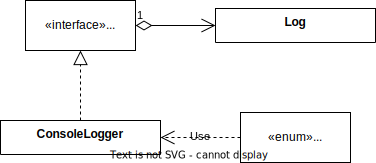
\includegraphics{img/日志类结构.svg}
    \caption{日志类的UML图}
\end{figure}

其中\codeline{ConsoleLogger}是内核中的一个日志输出器的实现。我们自己实现的日志输出器会替代它的位置。在实际使用日志时调用的是\codeline{Log}类,它包含一个\codeline{Logger},因此我们的日志输出器要实现\codeline{Logger}接口。\codeline{LogLevel}是日志的等级,如下表所示。

\begin{longtable}{p{2cm}|p{9cm}}
    日志等级 & 含义 \\
    \hline
    v & 冗长信息,指一般不需要过多关注,但是需要在日志中输出的信息\\
    \hline
    d & debug信息,建议在单元测试使用\\
    \hline
    i & 一般信息\\
    \hline
    w & 警告信息,比如传入的参数不规范,可能会导致报错时使用\\
    \hline
    e & 错误信息
\end{longtable}

\subsection[编写日志输出器]{编写日志输出器}\label{subsec:编写日志输出器}

编写日志输出器,首先要继承\codeline{Logger接口}并实现其中的所有方法。

\begin{lstlisting}[style=Java, caption={Logger初始布局},label={lst:Logger初始布局}]
public class MyLogger implements Logger
{
    @Override
    public void v(String tag, String message)
    {

    }

    @Override
    public void v(String tag, String message, Throwable throwable)
    {

    }
    // 其它方法
    // ...
}
\end{lstlisting}

每个方法的方法名都对应了日志等级。参数\codeline{String tag}是日志的标签,其作用是标记出给出日志的类。参数\codeline{String message}是日志的内容。参数\codeline{Throwable throwable}用于将报错的信息打印出来以便定位错误。这个参数是可选的,因为显然不一定所有日志都有报错信息。

这里给出\codeline{ConsoleLogger}的部分源码以供参考。

\begin{lstlisting}[style=Java, caption={ConsoleLogger源码},label={lst:ConsoleLogger源码}]
package com.potato.Log;

/**
 * ConsoleLogOutput是将日志输出至终端的一个实现
 */
public class ConsoleLogger implements Logger
{
    /**
     * 一般日志输出至标准输出流
     *
     * @param tag       用于分辨日志来源,可以设置为类名
     * @param message   日志信息
     * @param throwable 提供给日志的报错
     */
    private void normalPrintln(String tag, String message, Throwable throwable, LogLevel logLevel)
    {
        if (throwable != null)
        {
            System.out.printf("TAG:%s\t%s:%s\tTHROWABLE:%s%n", tag, logLevel, message, throwable);
        }
        else
        {
            System.out.printf("TAG:%s\t%s:%s%n", tag, logLevel, message);
        }
    }

    // 省略errorPrintln()的代码,它就是把normalPrintln()的out换成的err
    // 省略v()和d()的代码

    /**
     * 输出一般的信息
     *
     * @param tag     用于分辨日志来源,可以设置为类名
     * @param message 日志信息
     */
    @Override
    public void i(String tag, String message)
    {
        normalPrintln(tag, message, null, LogLevel.INFO);
    }

    /**
     * 输出一般的信息
     *
     * @param tag       用于分辨日志来源,可以设置为类名
     * @param message   日志信息
     * @param throwable 提供给日志的报错
     */
    @Override
    public void i(String tag, String message, Throwable throwable)
    {
        normalPrintln(tag, message, throwable, LogLevel.INFO);
    }

    // 省略w()的代码

    /**
     * 输出错误信息
     *
     * @param tag     用于分辨日志来源,可以设置为类名
     * @param message 日志信息
     */
    @Override
    public void e(String tag, String message)
    {
        errorPrintln(tag, message, null, LogLevel.ERROR);
    }

    /**
     * 输出错误信息
     *
     * @param tag       用于分辨日志来源,可以设置为类名
     * @param message   日志信息
     * @param throwable 提供给日志的报错
     */
    @Override
    public void e(String tag, String message, Throwable throwable)
    {
        errorPrintln(tag, message, throwable, LogLevel.ERROR);
    }
}

\end{lstlisting}

在编写完日志输出器后,在\codeline{Config}初始化时将\codeline{Logger logger}参数设置为自定义的日志输出器即可。

\begin{lstlisting}[style=Java, caption={设置日志输出器},label={lst:设置日志输出器}]
File configFile = // 配置文件
Config.initial(configFile, null, null, null, new MyLogger());
\end{lstlisting}


\end{document}
